\chapter{Подршка за екстерно дебаговање}

\рисцв{} стандард који прописује подршку за екстерно дебаговање \cite{debug_spec} предлаже следећу архитектуру система:

\begin{figure}[h!]
	\centering
	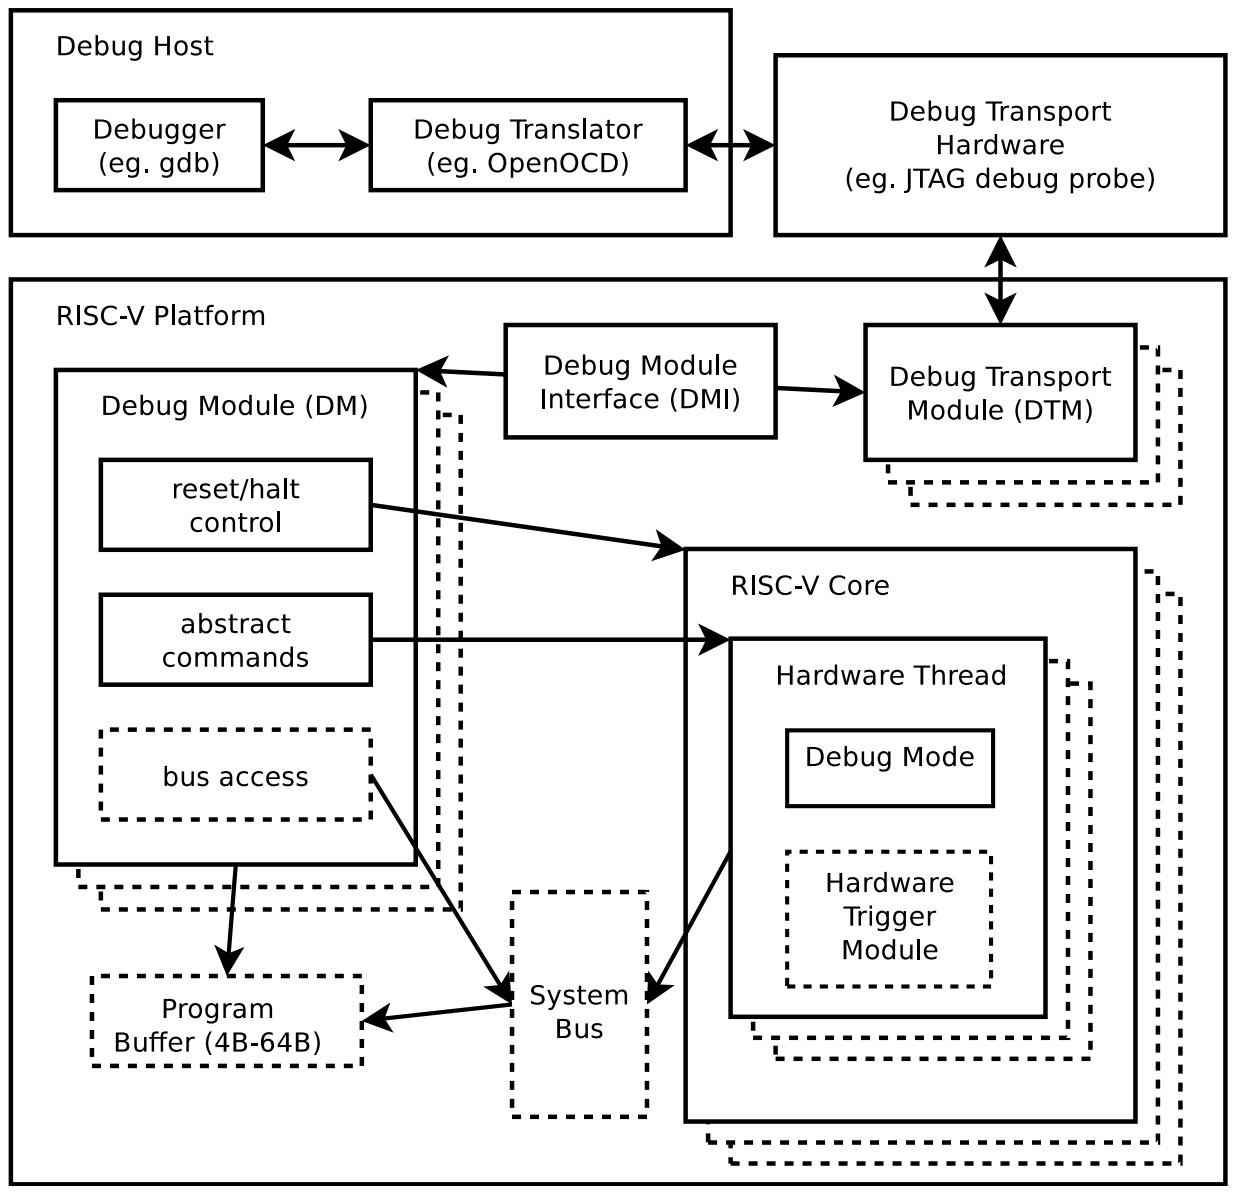
\includegraphics[width=0.7\textwidth]{arch}
	\caption{Предложена архитектура подршке за екстерно дебаговање \cite{debug_spec}}
	\label{fig:arch}
\end{figure}

Компоненте ван самог система и \дтм{} су објашњени у засебним поглављима, \textit{System Bus} се у контексту овог рада односи на \textit{Arilla bus} меморијску магистралу а \textit{Program Buffer} је имплементиран као део \дм{}-a. Преостале компоненте: \дм{}, \дми{}, интерфејс којим комуницирају језгро и \дм{}, потребне модификације језгра и хардверски окидачи су објашњене у остатку овог поглавља.

\дми{} је магистрала која повезује \дм{} и \дтм{}, и омогућава \дтм{}-у приступ адресном простору \дм{}-а. Спецификација подржава произвољну ширину адресе од минимално 7 бита, како један \дм{} заузима мање од 128 адреса, одабрана је минимална ширина адресне линије. \дми{} се састоји од: адресне линије, линије за податке и две контролне линије које означавају операције читања и уписа. Адресирање је на нивоу речи. Како \дм{} поседује релативно мали број регистара, могуће је комбинационо поставити одговарајућу вредност на линију за податке при операцији читања. Што омогућава магистрали да изврши једну операцију сваког такта, са кашњењем података од нула тактова при читању и упису. Како спецификација налаже да читање непостојећег регистра резултује читањем вредности 0, линија за податке унутар \дм{}-а (пре тростатичког бафера) је реализована као ожичено или.

\дм{} инкорпорира већину функционалности које дебагер користи за управљање језгром и увид у његово стање. Функционалности покретања и заустављања језгра, као и извршавање апстрактних команди су имплементиране коришћењем интерфејса који повезује \дм{} и језгро (дефинисаног у \textbf{debug\_if.svh}). Програмски бафер и приступ меморијској магистрали су реализовани меморијски мапираним регистрима и додатним контролером газде на магистрали респективно. 

Како би се подржало екстерно дебаговање неопходно је модификовати језгро. Модификације обухватају промене путање података и управљачке јединице, додавање контролних и статусних регистара и контролера језгра док је у режиму за дебаговање (компонента \textbf{D\_CTL}). Додатно унутар језгра се налазе и хардверски окидачи који при приступу одређеној адреси заустављају језгро и пребацују га у режим за дебаговање. 

Интерфејс који повезује \дм{} и језгро се састоји од следећих линија (прва половина представља линије у смеру од \дм{}-а ка језгру, а друга обратно):

\lstinputlisting[firstline = 4, lastline = 19,language=Verilog, caption=Линије \textbf{debug\_if} интерфејса]{../src/debug/debug_if.svh}

Линијама \textbf{halt\_req} и \textbf{resume\_req} \дм{} захтева од језгра да се заустави и настави са извршавањем респективно. Језгро повратну информацију о томе да ли је заустављено даје преко линије \textbf{halted}. Остатак линија се односи на извршавање апстрактних команди. У смеру од \дм{}-a ка језгру линија \textbf{exec} је активна од тренутка када дебагер захтева извршавање апстрактне команде све док језгро не обавести \дм{} да је команда извршена активном вредношћу линије \textbf{done}. Линије \textbf{command}, \textbf{data0\_in} и \textbf{data1\_in} садрже саму команду и њене потенцијалне аргументе, док линија \textbf{data0\_out} садржи резултат уколико постоји. Резултат се уписује у одговарајући регистар \дм{}-а када линија \textbf{write} има активну вредност.
Линије \textbf{bus}, \textbf{haltresume} и \textbf{exception} својом активном вредношћу сигнализирају да је дошло до одговарајуће грешке.\newpage

\section{\textit{\acrfull{DM}}}

\дм{} имплементира следеће регистре доступне преко \дми{} магистрале: \textbf{\acrshort{DMSTATUS}},\\ \textbf{\acrshort{DMCONTROL}}, \textbf{HARTINFO}, \textbf{\acrshort{HALTSUM}0}, \textbf{\acrshort{ABSTRACTCS}}, \textbf{COMMAND}, \textbf{ABSTRACTAUTO},\\ \textbf{\acrshort{SBCS}}, \textbf{\acrshort{SBADDRESS}0}, \textbf{\acrshort{SBDATA}0}, 12 \textbf{DATA} и 16 \textbf{\acrshort{PROGBUF}} регистара. \textbf{DATA} и \textbf{\acrshort{PROGBUF}} регистри су међусобно веома слични те се за њихово генерисање користе макрои налик онима коришћеним за контролне и статусне регистре. Регистри \textbf{DATA} и \textbf{\acrshort{PROGBUF}} су такође доступни језгру у виду меморијски мапираних регистара, за ово је наравно коришћена \textbf{periph\_mem\_interface} компонента.

\lstinputlisting[language=Verilog, caption=Пример макроа коришђених у \textbf{DM} компоненти,label={lst:dm}]{listing/debug.svh}

\subsection{Заустављање и поновно покретање језгра}

Заустављање и поновно покретање језгра, као и увид у то да ли је тренутно језгро заустављено је могуће кроз \textbf{\acrshort{DMSTATUS}} и \textbf{\acrshort{DMCONTROL}} регистре. Такође је могуће аутоматски зауставити језгро када се ресетује и то пре извршавања прве инструкције. Имплементација ових функционалности са стране \дм{}-а се у великој мери своди на повезивање одговарајућих бита \textbf{\acrshort{DMSTATUS}} и \textbf{\acrshort{DMCONTROL}} регистара на \textbf{debug\_if} интерфејс.

\subsection{Извршавање апстрактних команди}

Апстрактне команде омогућавају дебагеру да чита и пише регистре опште намене, контролне и статусне регистре и меморију, као и извршавање произвољног кода који се налази у \textbf{\acrshort{PROGBUF}} регистрима. Произвољан код је могуће извршити након или уместо приступа неком од регистара (коришћењем \textit{Access Register Command}) или \textit{Quick Access} командом која зауставља језгро, извршава произвољан код и поново покреће језгро. Апстрактна команда се извршава њеним уписом у \textbf{COMMAND} или уписом у \textbf{DATA} или \textbf{\acrshort{PROGBUF}} регистар чији је бит у \textbf{ABSTRACTAUTO} регистру постављен (ово поново извршава претходну команду са новим вредностима регистара). Команде користе \textbf{DATA} регистре за своје аргументе, по правилу  \textbf{DATA0}\footnote{Ово важи за системе са ширином речи од 32 бита, системи са већом ширином речи користе неколико узастопних регистара за један аргумент.} садржи вредност за упис или прочитану вредност док \textbf{DATA1} садржи меморијску адресу\footnote{Адреса регистра је енкодована директно у команди.}. \textbf{\acrshort{ABSTRACTCS}} регистар примарно садржи информацију о томе да ли је се апстрактна команда тренутно извршава и о грешци уколико је до ње дошло. Само мали део функционалности апстрактних команди је обавезан а приказана имплементација имплементира све опционе функционалности\footnote{Које су примењиве за имплементирано језгро.} осим приступа регистрима и меморији без заустављања језгра.

Већина инфраструктуре за извршавање апстрактних команди се налази у језгру, док је примарна улога \дм{}-а детекција одређених грешака. Грешке које \дм{} детектује су: покушај извршавања апстрактне команде док је извршавање апстрактне команде у току, извршавање апстрактних команди са неподржаним опцијама и извршавање команде која захтева да језгро буде заустављено уколико оно није. Док су грешке које детектује језгро: грешка при приступу меморији\footnote{Односи се само на приступ меморији помоћу апстрактних команди а не и на приступ помоћу газде на магистрали.}, извршавању невалидне инструкције или заустављању језгра из погрешног разлога. Поред пријављивања грешке, уписи у регистре који се тичу апстрактних команди док се апстрактна команда извршава немају ефекта. Такође уколико дође до грешке, није могуће извршавати апстрактне команде док се статус грешке не отклони уписивањем у  \textbf{\acrshort{ABSTRACTCS}} регистар. Након провере грешака коју врши \дм{}, он даје сигнал језгру да изврши апстрактну команду и прослеђује му саму команду и параметре. Језгро потом извршава команду и обавештава \дм{} када је извршена или уколико је дошло до грешке. Уколико команда уписује резултат у \textbf{DATA0} регистар, вредност и сигнал да је потребно извршити упис се такође прослеђују \дм{}-у. Уколико је команда успешно извршена и одговарајућа опција је подешена, \дм{} инкрементира одговарајућу адресу (уколико је у питању меморијска адреса уместо за један, регистар се инкрементира за величину приступа).

\subsection{Приступ меморији коришћењем додатног газде на магистрали}

Приступ меморији коришћењем додатног газде на магистрали је у потпуности имплементиран унутар \дм{}-а, без потребе за било каквим модификацијама језгра\footnote{Уколико је меморијски контролер у потпуности компатибилан са \textit{Arilla bus} магистралом.} и користи исти контролер меморије (компоненту \textbf{MEM\_INTERFACE}) само са различитим поларитетом линије \textbf{inhibit} који је подесив као параметар компоненте. Регистри \textbf{\acrshort{SBADDRESS}0} и \textbf{\acrshort{SBDATA}0} садрже адресу и вредност за приступ меморији а операције се започињу уписом или читањем неког од тих регистара у зависности од бита конфигурисаних у регистру \textbf{\acrshort{SBCS}}. Поред тога \textbf{\acrshort{SBCS}} садржи контролу величине приступа и инкрементирања адресе, као и бите који означавају да је дошло до грешке. Као и код апстрактних команди упис у \textbf{\acrshort{SBADDRESS}0} или \textbf{\acrshort{SBDATA}0} док је операција у току резултује у грешци и поред тога нема ефекат, слично операција се не може започети док се стање грешке не отклони уписом у одговарајуће бите \textbf{\acrshort{SBCS}} регистра. Остале грешке до којих може доћи су: приступ непостојећој меморији, лоше поравнат приступ меморији или неподржана величина приступа. При упису у регистар који започиње операцију постављају се бити који означавају да је операција започета (\textbf{sbbusy}) и тип операције (\textbf{sb\_read} или \textbf{sb\_write}).

Свака операција траје два такта, у првом такту (уколико није детектована грешка у величини приступа) се поставља активна вредност линије \textbf{inhibit} и обавља се приступ меморији.
У следећем такту се операција завршава уписом у \textbf{\acrshort{SBDATA}0} уколико је била реч о операцији читања и инкрементирањем адресе за величину приступа уколико је одговарајући бит подешен.

\section{Модификације језгра}

Како би подржало екстерно дебаговање неопходно је да језгро имплементира посебан мод извршавања (\textit{Debug} мод \textit{D}) и још неколико контролних и статусних регистара који обухватају \textbf{\acrshort{DCSR}}, \textbf{\acrshort{DPC}} и два помоћна регистра које дебагер може да користи за чување регистара опште намене. Језгро се налази у овом моду док је заустављено или извршава апстрактну команду. \textbf{\acrshort{DCSR}} регистар омогућава контролу над понашањем језгра док се налази у \textit{D} моду. Имплементирана поља овог регистра су:
\begin{itemize}
	\item \textbf{xdebugver} (само за читање), верзија спецификације за екстерно дебаговање коју језгро имплементира
	\item \textbf{ebreakm}, да ли \textbf{EBREAK} инструкција изазива изузетак или зауставља језгро
	\item \textbf{stepie}, да ли су прекиди омогућени у моду извршавања инструкцију по инструкцију
	\item \textbf{stopcount}, да ли су бројачи заустављени кад је језгро заустављено
	\item \textbf{stoptime}, да ли је тајмер заустављен кад је језгро заустављено
	\item \textbf{cause} (само за читање), разлог заустављања језгра
	\item \textbf{nmip} (само за читање), да ли постоји захтев за немаскирајући прекид
	\item \textbf{step}, да ли се језгро аутоматски зауставља након извршавања једне инструкције.
\end{itemize}
\textbf{\acrshort{DPC}} регистар памти вредност програмског бројача приликом уласка у \textit{D} мод и уписује ту вредност назад у програмски бројач при поновном покретању језгра (уписом у овај регистар је могуће променити локацију на којој ће језгро наставити извршавање). Сами регистри су имплементирани унутар \textbf{CSR} компоненте, као и логика која односи на заустављање бројача и тајмера. Остатак логике се претежно односи на прекиде и имплементиран је унутар \textbf{INT\_CTL} компоненте.

\subsection{Контролер режима за дебаговање}

Контролер режима за дебаговање (компонента \textbf{D\_CTL}) је повезан са \дм{}-ом путем \textbf{debug\_if} интерфејса и одговоран је за дистрибуцију тих информација остатку система.
Како би обезбедио заустављање система, контролер води рачуна о жељеном стању система на основу различитих сигнала који захтевају заустављање језгра, као што су: хардверски окидач окинут, извршена \textbf{EBREAK} инструкција\footnote{Уколико је \textbf{ebreakm} бит подешен.}, захтев за заустављање од стране \дм{}-а, заустављање након једне инструкције\footnote{Уколико је \textbf{step} бит подешен.} и извршавање \textit{Quick Access} апстрактне инструкције. Једини сигнал који може захтевати поновно покретање система је захтев од стране \дм{}-а. Контролер о овом жељеном стању обавештава управљачку јединицу а потом прати реално стање језгра на основу стања у коме се налази управљачка јединица и о том стању обавештава \дм{}, хардверске окидаче, контролер прекида и контролне и статусне регистре. При заустављању \textbf{D\_CTL} такође ажурира \textbf{\acrshort{DCSR}} кодом разлога заустављања и \textbf{\acrshort{DPC}} адресом од које се наставља извршавање (у случају да је разлог заустављање након једне инструкције или захтев од стране \дм{}-а бележи се адреса следеће инструкције\footnote{Уколико језгро није спремо да изврши тренутну инструкцију када добије захтев за заустављање, ипак се бележи тренутна адреса.}, у супротном се бележи адреса тренутне инструкције).
При извршавању апстрактних команди \textbf{D\_CTL} реконфигурише путању података како би управљачка јединица могла да манипулише регистрима и меморијом и води рачуна о извршавању произвољних инструкција враћањем оригиналне конфигурације путање података, скоком на програмски бафер и започињањем извршавања кода без напуштања \textit{D} мода. Како би успешно комуницирао са \дм{}-ом при извршавању апстрактних команди, контролер врши детекцију грешака и обавештава \дм{} о њима, као и о успешном завршетку извршавања апстрактне команде.

\subsection{Модификације путање података}

Како би се смањио број неопходних модификација путање података, одлучено је да се искористе исте линије које \textbf{INST\_DECODE} користи, што је реализовано инкорпорирањем декодовања апстрактних команди у \textbf{INST\_DECODE} тако да \textbf{D\_CTL} одређује да ли се декодује инструкција или апстрактна команда. Како се операциони кодови директно мапирају на стања управљачке јединице, за потребе апстрактних команди је уведено пет нових операционих кодова о којима ће бити више речи при опису модификација управљачке јединице.
Поред модификација \textbf{INST\_DECODE}-а, додати су нови улази у мултиплексере који одређују меморијску адресу и величину приступа меморији, додат је нови мултиплексер који одређује одакле долазе подаци који се уписују у меморију. Такође су додата два улаза у мултиплексер који одређује следећу адресу програмског бројача а то су: вредност \textbf{\acrshort{DPC}} регистра (користи се при поновном покретању језгра) и фиксна вредност локације почетка програмског бафера у меморијској мапи (користи се при извршавању произвољних инструкција).

\subsection{Модификације управљачке јединице}

На примеру кода \ref{lst:ctrls2} су приказана нова стања и контролне линије додате у односу на оне приказане у примеру \ref{lst:ctrls}.
Језгро се налази у стању \textbf{HALTED} када је заустављено и не извршава апстрактну команду, језгро улази у ово стање уколико је захтевано да се језгро заустави и прошли такт је био последњи такт инструкције или је језгро било у \textbf{PROLOGUE} стању. Језгро пролази кроз стање \textbf{RESUMING} при поновном покретању, тада се у програмски бројач уписује вредност \textbf{\acrshort{DPC}} регистра и језгро следећег такта прелази у \textbf{PROLOGUE} стање. Што значи да постоји кашњење од два такта од тренутка захтева за поновно покретање до провг такта извршавања инструкције.

\lstinputlisting[language=Verilog, caption=Додати контролни сигнали управљачке јединице,label={lst:ctrls2}]{listing/control_signals_if  copy.svh}

Остала нова стања се користе при извршавању апстрактних команди. У одговарајуће стање се улази када је језгро заустављено и \textbf{D\_CTL}
реконфигурише путању података, у које тачно стање се улази зависи од операционог кода декодованог у \textbf{INST\_DECODE}. \textbf{ABS\_REG} се користи за \textit{Access Register Command} уколико приступа регистрима, уколико само извршава програмски бафер или је у питању \textit{Quick Access}, језгро прелази у \textbf{ABS\_EXEC} стање, језгро такође може доћи у ово стање ако команда приступа регистрима и потом извршава програмски бафер. Уколико команда не приступа регистрима нити извршава програмски бафер (команда нема ефекта) језгро прелази у стање \textbf{ABS\_NA}. \textbf{ABS\_RMEM} и \textbf{ABS\_WMEM} се користе при читању и писању меморије. Као и при извршавању инструкција и при извршавању апстрактних команди, приступи меморији морају да се реализују кроз два такта чему служе стања \textbf{ABS\_RMEM\_1} и \textbf{ABS\_WMEM\_1}. Уколико је магистрала блокирана линијом \textbf{inhibit} (до чега у пракси не може доћи) како је једина разлика између стања \textbf{LOAD} и \textbf{LOAD\_W}\footnote{Исто важи и за стања \textbf{STORE} и \textbf{STORE\_W}.} била упис у инструкцијски регистар а \textbf{ABS\_RMEM} и \textbf{ABS\_WMEM} тај упис не врше, није потребно имати одвојена стања \textbf{ABS\_RMEM\_W} и \textbf{ABS\_WMEM\_W} већ је довољно да језгро остане у истом стању уколико приступ меморији није успео. Након извршене апстрактне команде, језгро се враћа у стање \textbf{HALTED}.\newpage

Како би управљачка јединица разликовала апстрактне команде које уписују или читају регистре, да ли су у питању регистри опште намене или контролни и статусни регистри, као и да ли се након приступа регистрима извршава програмски бафер, \textbf{INST\_DECODE} ове информације енкодује у линији \textbf{f3} којој сада и управљачка јединица има приступ. Линија \textbf{mcp\_addr} садржи тренутно стање управљачке јединице, овим се избегава додавање контролних сигнала који не учествују у путањи података а користе се у само једном стању. Ту функционалност екстензивно користе \textbf{INT\_CTL}, \textbf{D\_CTL} и \textbf{T\_CTL}. Сигналима \textbf{abstract\_write}, \textbf{abstract\_done} и \textbf{progbuf} управљачка јединица сигнализира \textbf{D\_CTL}-у да жели да упише резултат апстрактне команде у регистар, да је апстрактна команда извршена и да жели да почне са извршавањем програмског бафера респективно.

\lstinputlisting[firstline=153,lastline=197,language=Verilog, caption=Конфигурација контролих сигнала у додатим стањима управљачке јединице]{../src/core/control.sv}

\section{Хардверски окидачи}

Унутар језгра се налазе четири хардверска окидача који подржавају окидање на адресу или вредност приступа меморији (било да је у питању дохватање инструкције, упис или читање меморије). При окидању, језгро се зауставља, прелази у режим за дебаговање и обавештава \дм{} помоћу линије \textbf{halted}. Спецификација предвиђа осам контролних и статусних регистара кроз које се врши конфигурација окидача, од којих су 4 опциона и у овом случају неимплементирана. 
Имплементирани регистри су: \textbf{tdata1}, \textbf{tdata2}, \textbf{tinfo} и \textbf{tselect}. Сваки окидач има свој примерак прва три регистра, док регистар \textbf{tselect} одређује регистрима којег окидача се приступа. Регистар \textbf{tdata1} служи за конфигурацију окидача, подржане опције су: избор окидања на адресу или вредност приступа меморији\footnote{Вредност прочитана из или уписана у меморију.}, избор величине приступа меморији (8 бита, 16 бита, 32 бита или било која), избор окидања на било коју комбинацију дохватања инструкције, читања меморије и уписа у меморију. Регистар \textbf{tdata2} садржи вредност која се користи за поређење а \textbf{tinfo} је регистар намењен само за читање који садржи информацију о типовима окидача које тренутно изабран окидач подржава. Примећено је да тренутно доступни дебагери не проверавају овај регистар већ претпостављају да је једини подржан тип окидача наведен у регистру \textbf{tdata1}, ово онемогућава коришћење алтернативних типова окидача код окидача који подржавају више типова окидача, иако је то предвиђено спецификацијом.

Подршка за окидаче је имплементирана у компоненти \textbf{T\_CTL} која имплементира \textbf{tselect} регистар инстанцира одговарајући број окидача (компонента \textbf{TRIGGER}) и правилно мултиплексира регистре окидача у зависности од вредности \textbf{tselect} регистра. Како су у питању контролни и статусни регистри који се не налазе унутар \textbf{CSR} компоненте, раније приказан интерфејс који језгро користи за манипулацију контролним и статусним регистрима се користи у обрнутом смеру (при извршавању инструкције која модификује неки од ових регистара \textbf{CSR} поставља жељену вредност на линију \textbf{TDATA1\_in} активну вредност на линију \textbf{TDATA1\_write}\footnote{Исто важи и за регистре \textbf{tdata2} и \textbf{tselect}.}).
Овај \textbf{\_reg} \textbf{\_in} \textbf{\_write} интерфејс користи и сама компонента \textbf{TRIGGER} како би омогућила манипулацију својим регистрима. Што омогућава једноставно мултиплексирање регистара окидача повезивањем одговарајуће \textbf{\_in} линије свих окидача на \textbf{\_in} линију коју пружа интерфејс \textbf{CSR} компоненте, док се \textbf{\_write} линија повезује на израз формата \lstinline[columns=fixed]{csr_interface.TDATA1_write && tselect == i} где је \lstinline[columns=fixed]{i} индекс окидача.
Компонента \textbf{T\_CTL} такође формира глобални \textbf{trigger} сигнал дисјункцијом сигнала окидања свих окидача. \дм{} користи тај сигнал како би зауставио језгро када се неки од окидача окине.
Сам окидач (реализован у компоненти \textbf{TRIGGER}) имплементира \textbf{tdata1}, \textbf{tdata2} и \textbf{tinfo} регистре, логику која онемогућава упис неподржане конфигурације у регистре и саму логику за поређење и окидање која је реализована комбинационо.